%doc: Esteve/Photo Esteve.doc
\begin{news}
{2} %columnes
{Describe a Photo}
{\noindent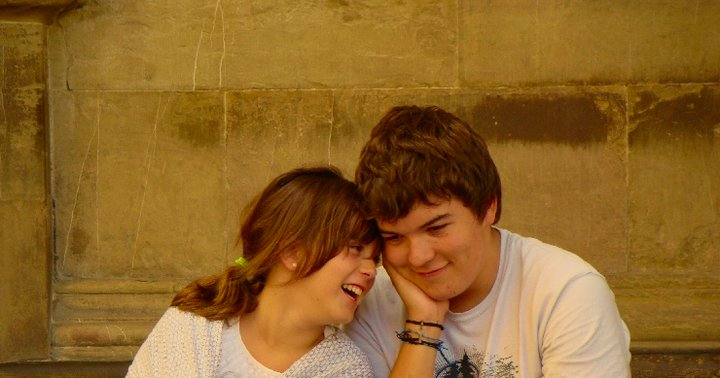
\includegraphics[width=18cm,keepaspectratio]{angles/img/foto_esteve.jpg}}
{Anglès}
{0501} %pagesof


This picture was taken two months ago, in a square in Florence

I was travelling with my parents and my sister around Italy. First we went to Venice and then to Florence, Siena and Pisa. In the picture my sister and me were talking about the Renaissance statues of the square called “Loggia de la Signoria”, a square with 25 statues on the street. We had been to that square more times because it was a moment of relax. But the best moment was one night when we were there before the dinner. Instead of a clown there was a musician with his guitar. He was playing songs that we all have in our memories, ans this was a really moving moment.

My parents love this photo because it's really natural ans spontaneous and it represents the friendship. My mum now has a two copies of the picture in the wall of her office. I am not always with my sister like in the picture. Not everything is always happy between us. Maybe this will be the Christmas postcard 2010.


\authorandplace{Esteve Pérez}{4th ESO}

\end{news}
